\section{Auswertung}
\label{sec:Auswertung}
\paragraph{Bestimmung des Polarisationswinkels}
Der im Versuchsaufbau verwedete Polarisationsfilter soll so eingestellt werden, dass maximaler Kontrast 
gewährleistet ist. Dazu wird der Winkel gegen den Kontrast aufgetragen und der Kontrast kann mit nicht-linearer 
Ausgleichrechnung bestimmt werden (vgl. Gleichung \eqref{eq:Kontrast2}). 
Damit kann dann der Winkel für den größten Kontrast bestimmt werden. Die 
Prozedur ist in der Abbildung \ref{fig:K} abgebildet. Der Polarisationswinkel mit größt möglichem Kontrast 
wurde zu $\theta \approx \SI{48}{\degree}$ bestimmt.
\begin{figure}
  \centering
  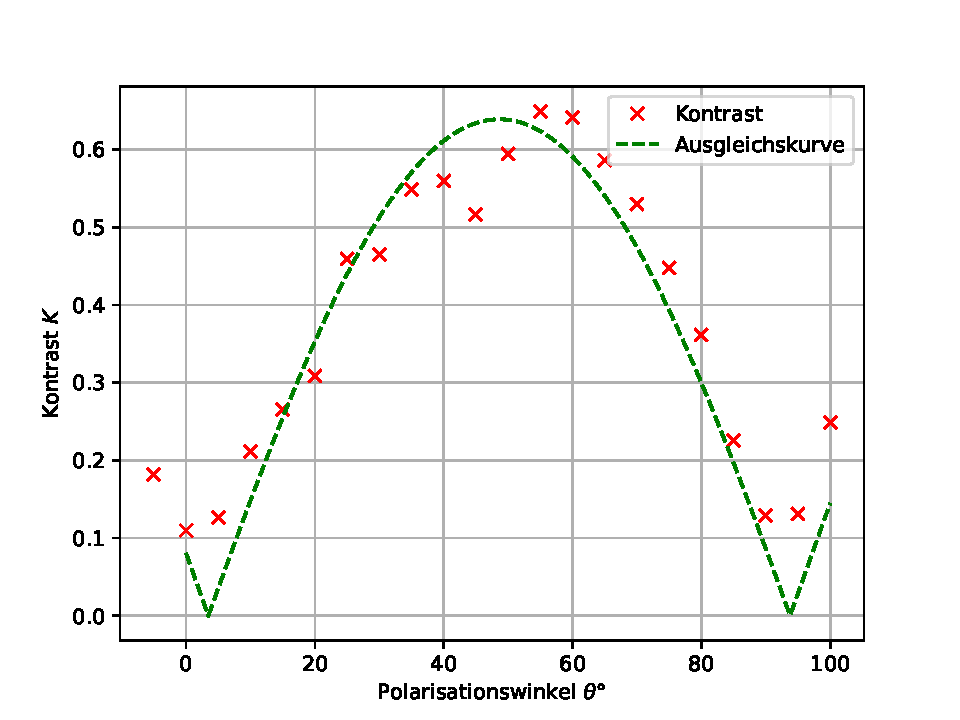
\includegraphics[height = 10cm]{plots/Kontrastfit.pdf}
  \caption{Kontrast aufgetragen gegen den Polarisationswinkel.}
  \label{fig:K}
\end{figure}
\FloatBarrier
\paragraph{Bestimmung des Brechungsindexes eines Glassplätchens}
Der Brechungindex in Abhängigkeit von der Anzahl der Interferenzmaxima ist gegeben über
\begin{equation}
M \approx \frac{2T}{\lambda_{vac}} \frac{n-1}{n} \delta \theta \;,
\label{eq:Mp}
\end{equation}
dabei bezeichnet $M$ die Anzahl, $T$ die Temperatur, $\lambda_{vac}$ die Vakuumwellenlänge und 
$\delta \theta$ die Winkeländerung.
Nun wird die Anzahl der Interferenzmaxima gegen die Winkeländerung aufgtreagenn und die Gleichung 
\eqref{eq:Mp} mit 
\begin{equation}
M = a \cdot \delta\theta \quad \text{mit} \quad a =M \approx \frac{2T}{\lambda_{vac}} \frac{n-1}{n}
\label{eq:pfit}
\end{equation}
approximiert und über Ausgleichrechnung der Paramter $a$ bestimmt. Das ist in der Abbildung 
\ref{fig:pfit} dargestellt. Die Daten dazu sind in der Tabelle \ref{tab:ptab} dargestellt.
\begin{figure}
  \centering
  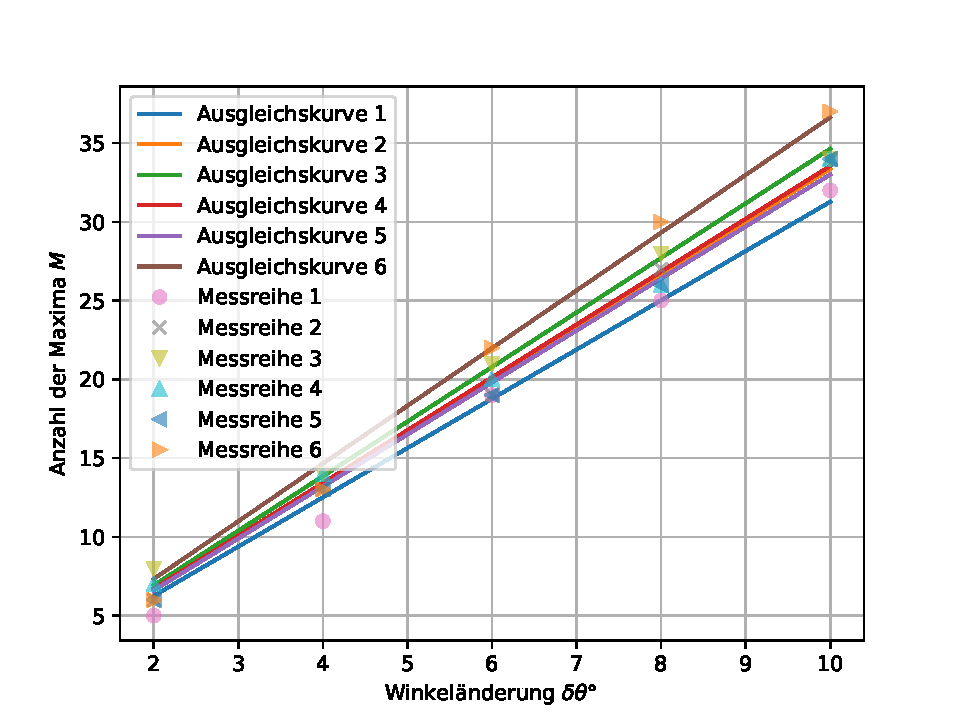
\includegraphics[height = 10cm]{plots/Plaettchenplot.pdf}
  \caption{Anzahl der Interferenzmaxima gegen die Winkeländerung aufgetragen für alle Messreihen.}
  \label{fig:pfit}
\end{figure}
\begin{table}
 \centering
 \sisetup{round-mode = places , round-precision = 0,scientific-notation=fixed, fixed-exponent = 0}
 % \resizebox{\textwidth}{!}{%
 \begin{tabular}{S@{${}\pm{}$} S}
   \toprule
    $\text{e}_b / \si{\milli\meter}$ &
    $\text{f}_b / \si{\milli\meter} $\\
   \midrule
   \bottomrule
 \end{tabular}
 % }
 \caption{Tabellenunterschrift}
 \label{tab:ptab}
\end{table}

\paragraph{Bestimmung des Brechungsindexes von Luft}
